\documentclass[11pt]{article}
\usepackage{acl-ijcnlp2009}
\usepackage{times}
\usepackage{latexsym}
\usepackage{prettyref}
\usepackage{subfig}
\usepackage{latexsym}
\usepackage{jeffe}
\usepackage{graphicx}
\usepackage{algorithm}
\usepackage[noend]{algpseudocode}
\usepackage{subfig}
\usepackage{hyphen}
\usepackage{relsize}
\usepackage[applemac]{inputenc}

\newrefformat{tab}{Table \ref{#1}} 
\newrefformat{fig}{Figure \ref{#1}} 
\newrefformat{eqn}{(\ref{#1})} 

\newcommand\bleu{${B{\scriptstyle LEU}}$}
\newcommand\boe{\mathbf{e}}
\newcommand\bof{\mathbf{f}}
\newcommand{\ind}[1]{{\fboxsep1pt\raisebox{-.5ex}{\fbox{{\tiny #1}}}}}
% allows margin notes
%\newcommand\margin[1]{} % hide them!!!
\newcommand\margin[1]{\mbox{}\marginpar{\raggedright\hspace{0pt}\tiny\em#1}}
\addtolength{\marginparwidth}{-3ex}

\setlength\titlebox{6.5cm}    % Expanding the titlebox

%% sloppy linebreaks
\sloppy

%% no extra spacing after dots
\frenchspacing

\makeatletter
\def\subsection{\@startsection{subsection}{2}{\z@}{-1.8ex plus
   -0.5ex minus -.2ex}{0.4ex plus .2ex}{\normalsize\bf\raggedright}}
\def\subsubsection{\@startsection{subsubsection}{3}{\z@}{1.5ex plus
  0.5ex minus .2ex}{0.2ex plus .1ex}{\normalsize\bf\raggedright}}
\def\paragraph{\@startsection{paragraph}{4}{\z@}{.75ex plus
  0.3ex minus .2ex}{-2em}{\normalsize\bf}}
\def\subparagraph{\@startsection{subparagraph}{5}{\parindent}{.75ex plus
  0.3ex minus .2ex}{-2em}{\normalsize\bf}}
\makeatother

% interline spacing
\renewcommand{\baselinestretch}{0.93}

\setlength{\textfloatsep}{3mm}
\setlength{\floatsep}{1.5mm}
\setlength{\dblfloatsep}{0.15cm}
\setlength{\dbltextfloatsep}{0.2cm}

\setlength{\intextsep}{0.15cm}
\setlength{\abovecaptionskip}{1mm}
\setlength{\topsep}{0mm}
\setlength{\partopsep}{0mm}

%\setlength{\columnsep}{3mm} % this one's nasty!!!


\title{A Note on the Implementation of \\ Hierarchical Dirichlet Processes}

\author{
  Phil Blunsom$^*$\\\vspace{6pt} pblunsom@inf.ed.ac.uk\\
  {\bf Sharon Goldwater$^*$}\\ sgwater@inf.ed.ac.uk
 \And
  Trevor Cohn$^*$\\\vspace{6pt} tcohn@inf.ed.ac.uk\\
  {\bf Mark Johnson$^\textrm{\textdagger}$}\\ mark\_johnson@brown.edu
 \AND
  {\rm $^*$Department of Informatics}\\
  University of Edinburgh\\
  Edinburgh, EH8 9AB, UK \And
  {\rm $^\textrm{\textdagger}$Department of Cognitive and Linguistic Sciences}\\
  Brown University \\
  Providence, RI, USA
}
\date{}

\begin{document}
\maketitle

% have to come after begin document
%\setlength{\parskip}{0mm}
\setlength{\abovedisplayskip}{1ex}
\setlength{\belowdisplayskip}{1ex}

\begin{abstract}
The implementation of collapsed Gibbs samplers for non-parametric Bayesian models is non-trivial, requiring considerable book-keeping.
\newcite{goldwater06} presented an approximation which significantly reduces the storage and computation overhead, but we show here that their formulation was incorrect and, even after correction, is grossly inaccurate. 
%Efficient implementation is of paramount importance for Gibbs samplers, but this is non-trivial for hierarchical Dirichlet process (HDP) models, which require considerable book-keeping.
%\newcite{goldwater06} presented an approximation which considerably reduces the storage and computation overhead, but we show here that their formulation was incorrect and even after correction is often grossly inaccurate. 
We present an alternative formulation which is exact and can be computed easily. 
However this approach does not work for hierarchical models, for which case we present an efficient data structure which has a better space complexity than the naive approach.  
\end{abstract}

\section{Introduction}
Unsupervised learning of natural language is one of the most challenging areas in NLP.  
Recently, methods from nonparametric Bayesian statistics have been gaining popularity as a way to approach unsupervised learning for a variety of tasks, including language modeling, word and morpheme segmentation, parsing, and machine translation \cite{teh06hdp,goldwater06,goldwater06interpolating,liang07hdppcfg,finkel07infinite,denero08sampling}. %,blunsom08bscfg}.  
These models are often based on the Dirichlet process (DP) \cite{ferguson73} or hierarchical Dirichlet process (HDP) \cite{teh06hdp}, with Gibbs sampling as a method of inference.  
Exact implementation of such sampling methods requires considerable bookkeeping of various counts, which motivated \newcite{goldwater06} (henceforth, GGJ06) to develop an approximation using expected counts.  
However, we show here that their approximation is flawed in two respects: 1) It omits an important factor in the expectation, and 2) Even after correction, the approximation is poor for hierarchical models, which are commonly used for NLP applications.  
We derive an improved  
$\mathcal{O}(1)$ formula that gives exact values for the expected counts in non-hierarchical models.  For hierarchical models, where our formula is not exact, 
% approximation formula and show that it follows empirical values much more tightly in a wider variety of settings.  For settings in which the approximation is inappropriate, 
we present an efficient method for sampling from the HDP (and related
models, such as the hierarchical Pitman-Yor process) that considerably decreases
the memory footprint of such models as compared to the naive
implementation.

As we have noted, the issues described in this paper apply to models for various kinds of NLP tasks; for concreteness, we will focus on $n$-gram language modeling for the remainder of the paper, closely following the presentation in GGJ06.

\vspace{-0.05in}
\section{The Chinese Restaurant Process}
GGJ06 present two nonparametric Bayesian language models: a DP unigram
model and an HDP bigram model. Under the DP model, words in a corpus
$\mathbf{w} = w_1 \ldots w_n$ are generated as follows: 
\begin{align}
\nonumber G | & \alpha_0, P_0 & \sim & ~ \mbox{DP}(\alpha_0,P_0) \\
\nonumber w_i | & G & \sim & ~ G 
\end{align}
where $G$ is a distribution over an infinite set of possible words,
$P_0$ (the {\em base distribution} of the DP) determines the
probability that an item will be in the support of $G$, and $\alpha_0$
(the {\em concentration parameter}) determines the variance of $G$.

One way of understanding the predictions that the DP model makes is through the Chinese restaurant process (CRP)
\cite{aldous85}. 
In the CRP, customers (word tokens $w_i$) enter a restaurant with an infinite number of tables and choose a seat.  
The table chosen by the $i$th customer, $z_i$, follows the distribution:
\begin{align}
\nonumber P(z_i = k | \mathbf{z}_{-i}) = \left\{ 
\begin{array}{ll} 
  \frac{n_k^{\mathbf{z}_{-i}}}{i - 1 + \alpha_0}, 0 \leq k < K(\mathbf{z}_{-i}) \\
  \frac{\alpha_0}{i - 1 + \alpha_0}, k = K(\mathbf{z}_{-i})
\end{array} \right.
\label{eqn:crp}
\end{align}
where $\mathbf{z}_{-i} = z_1 \dots z_{i-1}$ are the table assignments of the previous customers, $n_k^{\mathbf{z}_{-i}}$ is the number of customers at table $k$ in ${\mathbf{z}_{-i}}$, and $K(\mathbf{z}_{-i})$ is
the total number of occupied tables.  
If we further assume that table $k$ is labeled with a word type $\ell_k$ drawn from $P_0$, then the assignment of tokens to tables defines a distribution over words, with $w_i = \ell_{z_i}$.
See Figure \ref{fig:tables} for an example seating arrangement.  

\begin{figure}
\begin{center}
\includegraphics[width=1.0\columnwidth]{tables.pdf}
\end{center}
\caption[]{A seating assignment describing the state of a unigram CRP. Letters and numbers uniquely identify customers and tables. Note that multiple tables may share a label.}
\label{fig:tables}
\end{figure}


Using this model, the predictive probability of $w_i$, conditioned on
the previous words, can be found by summing over possible seating
assignments for $w_i$, and is given by
\begin{align}
P(w_i = w | \mathbf{w}_{-i}) = \frac{n_{w}^{\mathbf{w}_{-i}} + \alpha_0 P_0}{i-1 + \alpha_0}
\end{align}
This prediction turns out to be exactly that of the DP model after integrating out the distribution $G$.  
Note that as long as the base distribution $P_0$ is fixed, predictions do not depend on the seating arrangement $\mathbf{z}_{-i}$, only on the count of word $w$ in the previously observed words ($n_{w}^{\mathbf{w}_{-i}}$).  
However, in many situations, we may wish to estimate the base distribution itself, creating a {\em hierarchical} model.  
Since the base distribution generates table labels, estimates of this distribution are based on the counts of those labels, i.e., the number of tables associated with each word type.

An example of such a hierarchical model is the HDP bigram model of
GGJ06, in which each word type $w$ is associated with its own
restaurant, where customers in that restaurant correspond to words
that follow $w$ in the corpus. All the bigram restaurants share a
common base distribution $P_1$ over unigrams, which must be inferred.
Predictions in this model are as follows:
\begin{align}
\small
\nonumber P_2(w_i | \mathbf{h}_{-i}) &= \frac{n_{(w_{i-1},w_i)}^{\mathbf{h_{-i}}} + \alpha_1 P_1(w_i | \mathbf{h}_{-i})}{n_{(w_{i-1}, *)}^{\mathbf{h_{-i}}} + \alpha_1} \\
 P_1(w_i | \mathbf{h}_{-i}) &= %\left\{ 
  \frac{t_{w_i}^{\mathbf{h_{-i}}} + \alpha_0 P_0(w_i)}{t_*^{\mathbf{h_{-i}}} + \alpha_0} \label{eq:hdp_p1}
%\begin{array}{ll} 
%  \frac{t_{\Sigma*} + \frac{\tau}{2}}{t + \tau} \frac{t_{w_i} + \alpha_0 P_0(w_i)}{t_{\Sigma*} + \alpha_0}, w_i \in \Sigma* 
%  \frac{t_{\Sigma*} + \frac{\tau}{2}}{t + \tau}, w_i = \$
%\end{array} \right.
\end{align}
where $\mathbf{h}_{-i} = (\mathbf{w}_{-i}, \mathbf{z}_{-i})$, $t_{w_i}^{\mathbf{h_{-i}}}$ is the number of tables labelled with $w_i$, and $t_*^{\mathbf{h_{-i}}}$ is the total number of occupied tables.
Of particular note for our discussion is that in order to calculate these conditional distributions we must know the table assignments $\mathbf{z}_{-i}$ for each of the words in $\mathbf{w}_{-i}$.  Moreover, in the Gibbs samplers often used for inference in these kinds of models, the counts are constantly changing over multiple samples, with tables going in and out of existence frequently.  This can create significant bookkeeping issues in implementation, and motivated GGJ06 to present a method of computing approximate table counts based on word frequencies only.

\section{Approximating Table Counts}
\begin{figure}[t]
\begin{center}
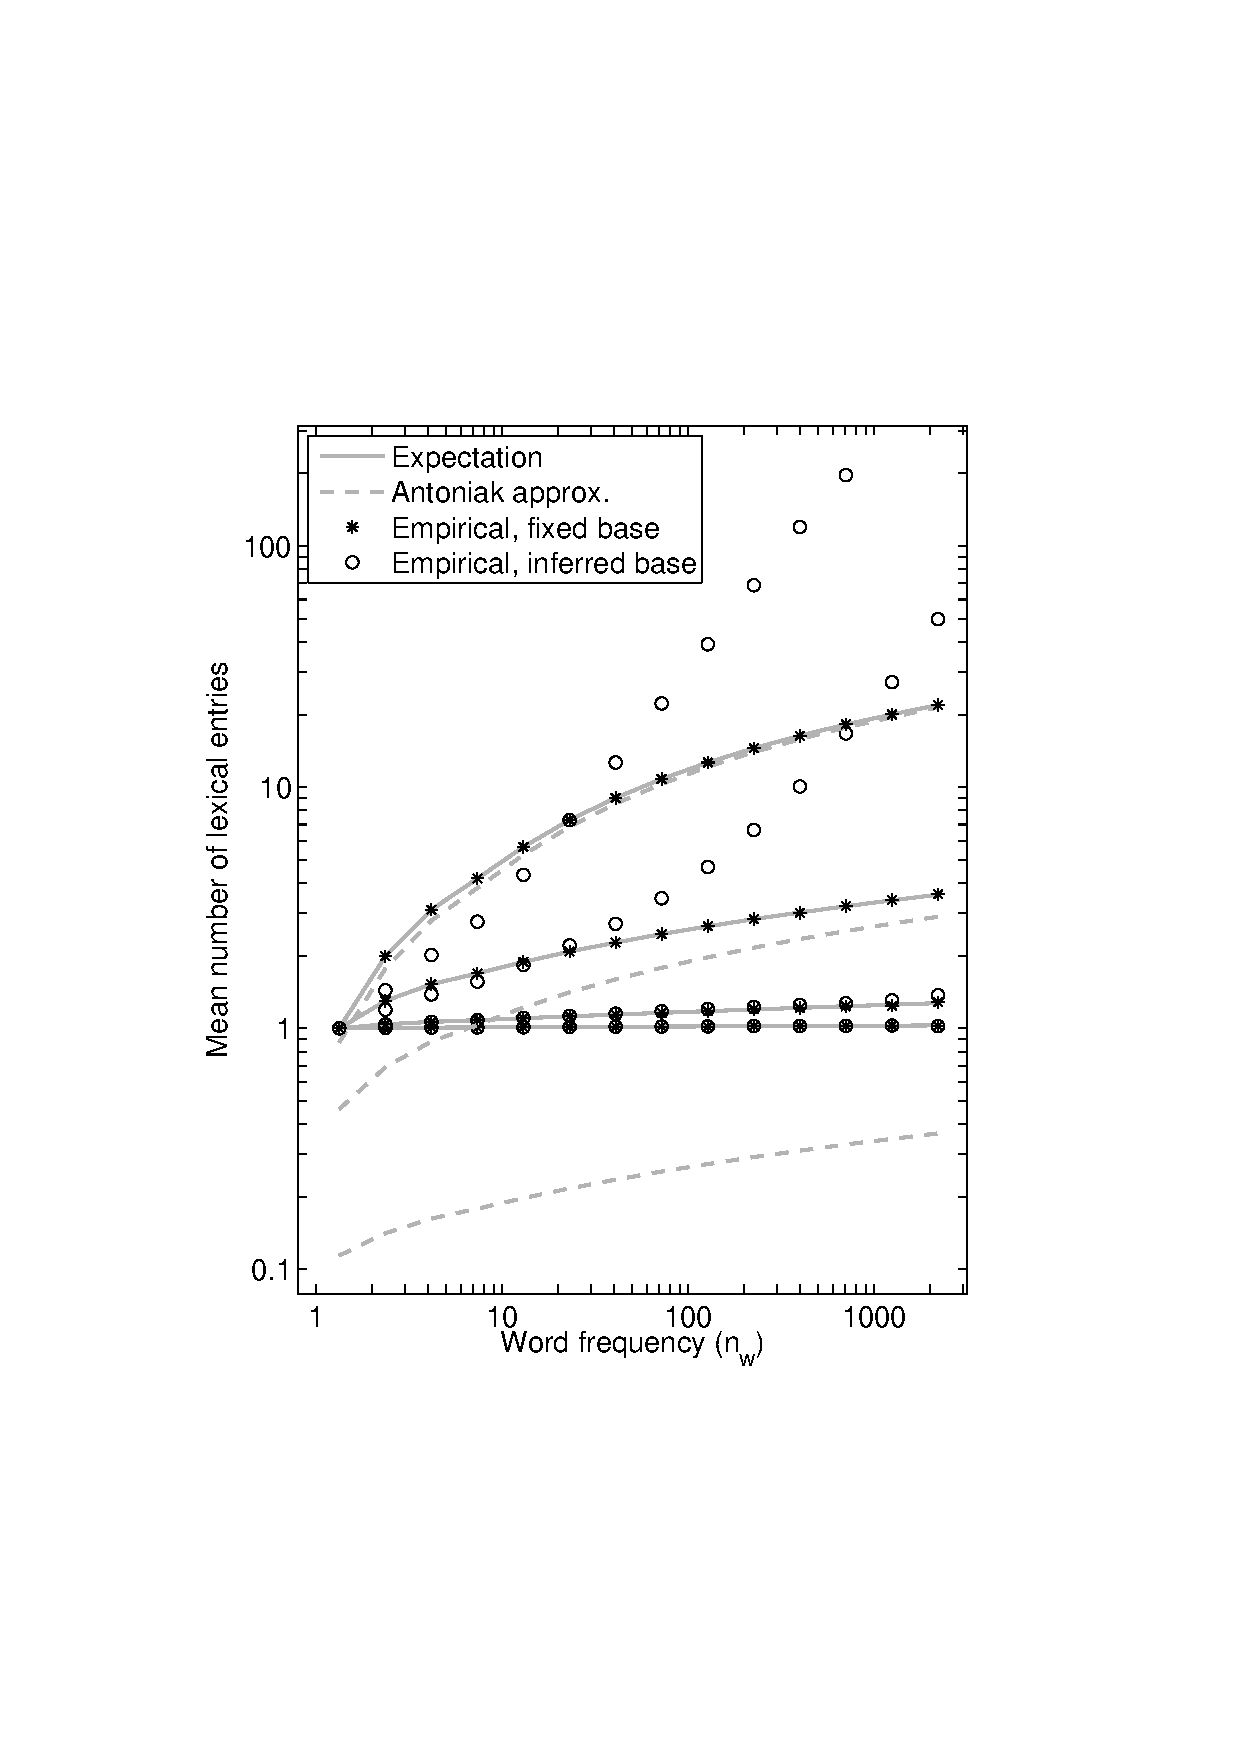
\includegraphics[scale=0.5]{approximations.pdf}
\end{center}
\caption[]{Comparison of several methods of approximating the number of tables occupied by words of different frequencies. 
For each method, results using $\alpha = \{100, 1000, 10000, 100000\}$ are shown (from bottom to top).  
Solid lines show the expected number of tables, computed using (\ref{eqn:true_expected}) and assuming $P_1$ is a fixed uniform distribution over a finite vocabulary (values computed using the Digamma formulation (\ref{eqn:digamma}) are the same).    
Dashed lines show the values given by the Antoniak approximation (\ref{eqn:antoniak_approximation}) (the line for $\alpha = 100$ falls below the bottom of the graph).  
Stars show the mean of empirical table counts as computed over 1000 samples from an MCMC sampler in which $P_1$ is a fixed uniform distribution, as in the unigram LM.  
Circles show the mean of empirical table counts when $P_1$ is inferred, as in the bigram LM.  Standard errors in both cases are no larger than the marker size.  
All plots are based on the 30114-word vocabulary and frequencies found in sections 0-20 of the WSJ corpus.}
\label{fig:graphs}
\end{figure}

Rather than explicitly tracking the number of tables $t_w$ associated with each word $w$ in their bigram model,  GGJ06 approximate the table counts using the expectation $E[t_{w}]$. Expected counts are used in place of $t_{w_i}^{\mathbf{h_{-i}}}$  and $t_*^{\mathbf{h_{-i}}}$ in~(\ref{eq:hdp_p1}).  The exact expectation, due to \newcite{antoniak74}, is
\begin{align}
E[t_w] = \alpha_1 P_1(w) \sum_{i=1}^{n_w} \frac{1}{\alpha_1 P_1(w) + i - 1}
\label{eqn:true_expected}
\end{align}
Antoniak also gives an approximation to this expectation:
\begin{align}
E[t_w] \approx \alpha_1 P_1(w) \log \frac{n_w + \alpha_1 P_1(w)}{\alpha_1 P_1(w)}
\label{eqn:antoniak_approximation}
\end{align}
but provides no derivation.  Due to a misinterpretation of  \newcite{antoniak74}, GGJ06 use an approximation that leaves out all the $P_1(w)$ terms from (\ref{eqn:antoniak_approximation}).\footnote{The authors of GGJ06 realized this error, and current implementations of their models no longer use these approximations, instead tracking table counts explicitly.}  
Figure \ref{fig:graphs} compares the approximation to the exact expectation when the base distribution is fixed.  The approximation is fairly good when $\alpha P_1(w) > 1$ (the scenario assumed by Antoniak); however, in most NLP applications, $\alpha P_1(w) < 1$ in order to  effect a sparse prior.  (We return to the case of non-fixed based distributions in a moment.)
As an extreme case of the paucity of this approximation consider $\alpha_1 P_1(w) = 1$ and $n_w=1$ (i.e. only one customer has entered the restaurant): clearly $E[t_w]$ should equal $1$, but the approximation gives $log(2)$.


We now provide a derivation for (\ref{eqn:antoniak_approximation}), which will allow us to obtain an  $\mathcal{O}(1)$ formula for the expectation in (\ref{eqn:true_expected}).  First, we rewrite the summation in (\ref{eqn:true_expected}) as a difference of fractional harmonic numbers:\footnote{Fractional harmonic numbers between 0 and 1 are given by $ H_F =\int_0^1 \frac{1 -x^F} {1 -x} dx$.  All harmonic numbers follow the recurrence $H_F = H_{F-1} + \frac{1}{F}$.}
\begin{align}
\label{eqn:harmonic}
%\!\!\!\! E[t_w] = \alpha_1 P_1(w) \Big [ H_{(\alpha_1 P_1(w)+n_w-1)} - H_{(\alpha_1 P_1(w)-1)} \Big ]
 H_{(\alpha_1 P_1(w)+n_w-1)} - H_{(\alpha_1 P_1(w)-1)}
\end{align}
Using the recurrence for harmonic numbers:
%\end{equation*}
\begin{multline}
\!\!\!\!\!\! E[t_w] \approx \alpha_1 P_1(w) \Big[ H_{(\alpha_1 P_1(w)+n_w)} - \frac{1}{\alpha_1 P_1(w)+n_w}\\  - H_{(\alpha_1 P_1(w) + n_w)} + \frac{1}{\alpha_1 P_1(w)} \Big ]
\end{multline}
We then use the asymptotic expansion, \mbox{$H_F \approx \log{F} + \gamma + \frac{1}{2F}$}, omiting trailing terms which are $\mathcal{O}(F^{-2})$ and smaller powers of $F$:\footnote{Here, $\gamma$ is the Euler-Mascheroni constant.}
\begin{equation*}
\mathsmaller{E[t_w] \approx \alpha_1 P_1(w) \log \frac{n_w + \alpha_1 P_1(w)}{\alpha_1 P_1(w)} + \frac{n_w}{2(\alpha_1 P_1(w)+n_w)}}
%\label{eqn:harm_approx}
\end{equation*}

Omitting the trailing term leads to the approximation in \newcite{antoniak74}.  
However, we can obtain an exact formula for the expectation by 
utilising the relationship between the Digamma function and the harmonic numbers: \mbox{$\psi(n) = H_{n-1} - \gamma$}.\footnote{Accurate $\mathcal{O}(1)$ approximations of the Digamma function are readily available.}
Thus we can rewrite (\ref{eqn:harmonic}) as:\footnote{(\ref{eqn:digamma}) can be derived from (\ref{eqn:true_expected}) using: $\psi(x+1) - \psi(x) = \frac{1}{x}$.}
%\begin{equation}
\begin{multline}
%\mathsmaller{
E[t_w] = \alpha_1 P_1(w) \cdot \\
 \big [\psi{(\alpha_1 P_1(w)+n_w)} - \psi{(\alpha_1 P_1(w)}) \big ]
\label{eqn:digamma}
%}
\end{multline}
%\end{equation}

%The mean squared error of Eq.~\ref{eqn:antoniak_approximation} over the range $1\times10^{-4} < \alpha P_0(w) < 1$ in $1\times10^{-4}$ increments, and $n_w \in [1,20]$, is $1.38$. For Eq.~\ref{eqn:harmonic} with the extra expansion terms it's $0.14$, while with the Digamma function it's $6\times10^{-29}$.
%Figure \ref{fig:graphs} compares empirically observed table counts with their exact and approximate expectations, clearly showing the poor quality of the GGJ06 approximation.

A significant caveat here is that the expected table counts given by (\ref{eqn:true_expected}) and (\ref{eqn:digamma}) are only valid when the base distribution is a constant.  However, in hierarchical models such as GGJ06's bigram model and HDP models, the base distribution is not constant and instead must be inferred.  As can be seen in Figure~\ref{fig:graphs}, table counts can diverge considerably from the expectations based on fixed $P_1$ when $P_1$ is in fact not fixed.  Thus,  (\ref{eqn:digamma}) can be viewed as an approximation in this case, but not necessarily an accurate one.  Since knowing the table counts is only necessary for inference in hierarchical models, but the table counts cannot be approximated well by any of the formulas presented here, we must conclude that the best inference method is still to keep track of the actual table counts.  The naive method of doing so is to store which table each customer in the restaurant is seated at, incrementing and decrementing these counts as needed during the sampling process.  In the following section, we describe an alternative method that reduces the amount of memory necessary for implementing HDPs.  This method is also appropriate for hierarchical Pitman-Yor processes, for which no closed-form approximations to the table counts have been proposed.


\section{Efficient Implementation of HDPs}

As we do not have an efficient expected table count approximation for hierarchical models we could fall back to explicitly tracking which table each customer that enters the restaurant sits at.
However, here we describe a more compact representation for the state of the restaurant that doesn't require explicit table tracking.\footnote{\newcite{teh06hdp} also note that the exact table assignments for customers are not required for prediction.}
Instead we maintain a histogram for each dish $w_i$ of the frequency of a table having a particular number of customers.
Figure \ref{fig:histogram} depicts the histogram and explicit representations for the CRP state in Figure \ref{fig:tables}.

\begin{figure}
%\begin{center}
%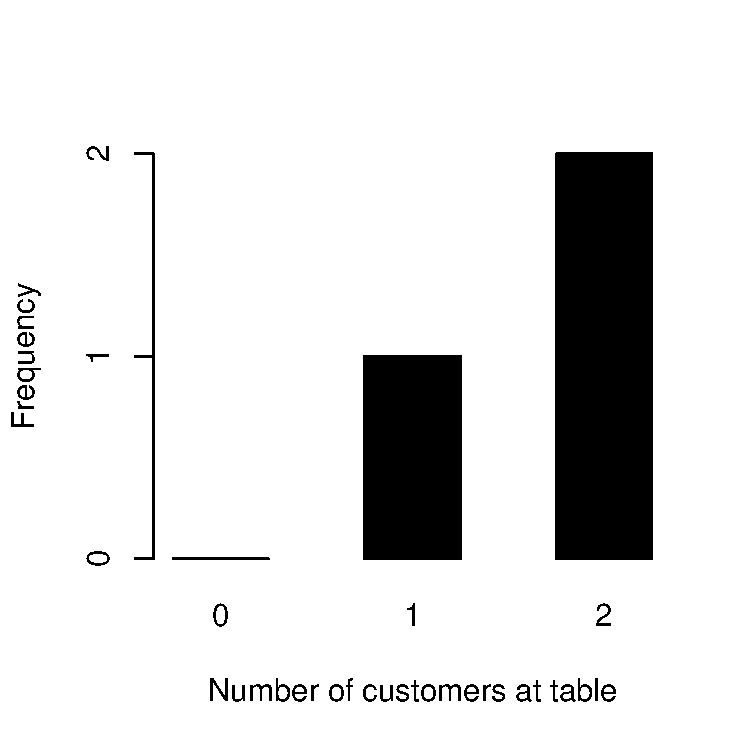
\includegraphics[width=0.8\columnwidth]{tables_histogram.pdf}
%\end{center}
\begin{tabular}{l}
{\bf Explicit table tracking:} \\
customer($w_i$) $\rightarrow$ table($z_i$) \\
{\small $\Big \{a:1,\ b:1,\ c:2,\ d:2,\ e:3,\ f:4,\ g:5,\ h:5 \Big \}$} \\
table($z_i$) $\rightarrow$ label($\ell$) \\
{\small $\Big \{1: The,\ 2: cats,\ 3: cats,\ 4: meow,\ 5: cats \Big \} $}
\vspace{0.05cm} \\
\bf{Histogram:} \\
word type $\rightarrow \Big \{$ table occupancy $\rightarrow$ frequency $\Big \}$ \\
{\small $\Big \{\ The : \{2:1\},\ cats : \{1:1,\ 2:2\},\ meow : \{1:1\} \Big \}$} \\
\end{tabular}

\caption[]{The explicit table tracking and histogram representations for Figure \ref{fig:tables}.}
\label{fig:histogram}
\end{figure}

Our alternative method of inference for hierarchical Bayesian models takes advantage of their exchangeability, which makes it unnecessary to know exactly which table each customer is seated at.  The only important information is how many tables exist with different numbers of customers, and what their labels are.  We simply maintain a histogram for each word type $w$, which stores, for each number of customers $m$, the number of tables labeled with $w$ that have $m$ customers.
Figure \ref{fig:histogram} depicts the explicit representation and histogram for the CRP state in Figure \ref{fig:tables}.

Algorithms \ref{alg:increment} and \ref{alg:decrement} describe the two operations required to maintain the state of a CRP.\footnote{A C++ template class that implements the algorithm presented is made available at: {http://homepages.inf.ed.ac.uk/tcohn/}}
When a customer enters the restaurant (Alogrithm \ref{alg:increment})), we sample whether or not to open a new table.  If not, we sample an old table proportional to the counts of how many customers are seated there and update the histogram.  When a customer leaves the restaurant (Algorithm \ref{alg:decrement}), we decrement one of the tables at random according to the number of customers seated there.  By exchangeability, it doesn't actually matter which table the customer was ``really" sitting at.

\begin{algorithm}[t]
\caption{A new customer enters the restaurant}
\begin{small}
\begin{algorithmic}[1]
\State $w$: word type
\State $P_0^w$: Base probability for $w$ 
\State $\mbox{HD}_w$: Seating Histogram for $w$
\Procedure{\footnotesize INCREMENT}{$w, P_0^{w}, \mbox{HD}_w$} 

  \State $p_{share} \gets \frac{n_{w}^{\mathbf{w}_{-1}}}{n_{w}^{\mathbf{w}_{-1}} + \alpha_0}$ \Comment{share an existing table}
  \State $p_{new} \gets \frac{\alpha_0 \times P_0^{w}}{n_{w}^{\mathbf{w}_{-1}} + \alpha_0}$ \Comment{open a new table}

  \State $r \gets random(0, p_{share} + p_{new})$ 
  \If{$r < p_{new}\ \mbox{or}\ n_{w}^{\mathbf{w}_{-1}} = 0$}
    \State $\mbox{HD}_w[1] = \mbox{HD}_w[1] + 1$
  \Else 
    \Statex \Comment{Sample from the histogram of customers at tables}
    \State $r \gets random(0, n_{w}^{\mathbf{w}_{-1}})$ 
    \For{$c \in \mbox{HD}_w$} \Comment{$c$: customer count}
      \State $r = r - (c \times \mbox{HD}_w[c])$ 
      \If{$r \leq 0$}
        \State $\mbox{HD}_w[c] = \mbox{HD}_w[c] + 1$
        \State Break
      \EndIf
    \EndFor
  \EndIf
  \State $n_{w}^{\mathbf{w}} = n_{w}^{\mathbf{w}_{-1}} + 1$ \Comment{Update token count}
\EndProcedure
\end{algorithmic}
\end{small}
\label{alg:increment}
\end{algorithm}

\begin{algorithm}[t]
\caption{A customer leaves the restaurant}
\begin{small}
\begin{algorithmic}[1]
\State $w$: word type
\State $\mbox{HD}_w$: Seating histogram for $w$
\Procedure{\footnotesize DECREMENT}{$w, P_0^{w}, \mbox{HD}_w$} 
  \State $r \gets random(0, n_{w}^{\mathbf{w}})$ 
  \For{$c \in \mbox{HD}_w$} \Comment{$c$: customer count}
    \State $r = r - (c \times \mbox{HD}_w[c])$ 
    \If{$r \leq 0$}
      \State $\mbox{HD}_w[c] = \mbox{HD}_w[c] - 1$
      \If{$c > 1$}
        \State $\mbox{HD}_w[c - 1] = \mbox{HD}_w[c - 1] + 1$
      \EndIf
      \State Break
    \EndIf
  \EndFor
  \State $n_{w}^{\mathbf{w}} = n_{w}^{\mathbf{w}} - 1$ \Comment{Update token count}
\EndProcedure
\end{algorithmic}
\end{small}
\label{alg:decrement}
\end{algorithm}

%\vspace{-0.05in}
\section{Conclusion}
We've shown that the \mbox{HD}P approximation presented in GGJ06 contained errors and inappropriate assumptions such that it significantly diverges from the true expectations for the most common scenarios encountered in NLP.
As such we emphasise that that formulation should not be used.
Although (\ref{eqn:digamma}) allows $E[t_w]$ to be calculated exactly for constant base distributions, for hierarchical models this is not valid and no accurate calculation of the expectations has been proposed. 
As a remedy we've presented an algorithm that efficiently implements the true \mbox{HD}P without the need for explicitly tracking customer to table assignments, while remaining simple to implement.


\section*{Acknowledgements}
The authors would like to thank Tom Griffiths for providing the code used to produce Figure \ref{fig:graphs} and acknowledge the support of the EPSRC (Blunsom, grant EP/D074959/1; Cohn, grant GR/T04557/01).


\bibliographystyle{scrunchacl}
\newcommand{\bibsnip}{\vspace{-1ex}}
\begin{small}
\bibliography{standard}
\end{small}

\end{document}
